
\documentclass{llncs}
%
% additional packages added to comply wth format recommendations
%
\usepackage{makeidx}  % allows for indexgeneration
\usepackage[strings]{underscore} % allows underscore
\usepackage{float} % position tables inline
\usepackage{placeins}
\usepackage{caption}
\captionsetup[table]{singlelinecheck=false,
					labelfont=bf,
					justification=raggedright,
					labelsep=period}
\usepackage{textcomp}
\usepackage{colortbl}
\usepackage{graphicx}


% ... -=-=-=-=-=-=-=-=-=-=-=-=-=-=-=-=-=-=-=-=-=-=-=-=-=-=-=-=-=-=-=-=-=-=-=-=-
% ...	 directory paths for images
% ... -=-=-=-=-=-=-=-=-=-=-=-=-=-=-=-=-=-=-=-=-=-=-=-=-=-=-=-=-=-=-=-=-=-=-=-=-

\graphicspath{
    {.} % document root dir
    {images/}
}


%\usepackage{subcaption}		% enables side-by-side figures
%\captionsetup{compatibility = false}	% needed for subcaption package

\begin{document}

the below double figure ~\ref{figure : dataFeatureDevelopment}.

\begin{center}
This is a pseudo-caption.\newline
\label{fig : dataFeatureDevelopment}
  \begin{tabular}{ *{2}{c} }
    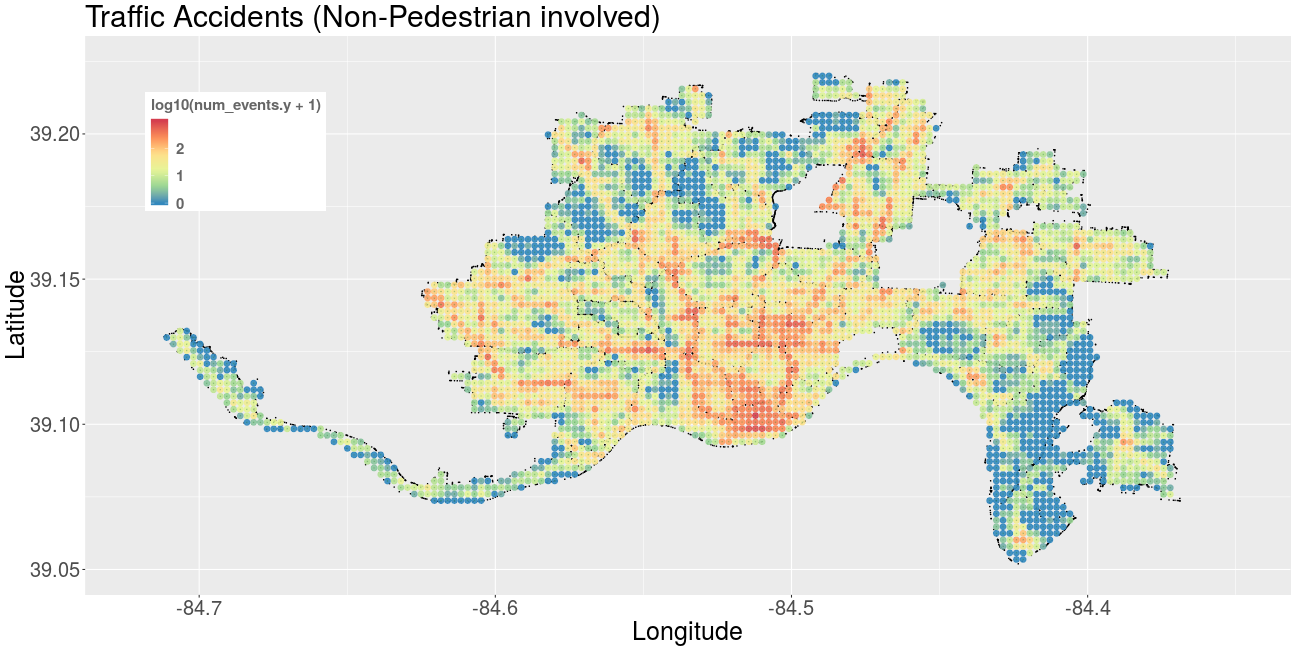
\includegraphics[height=3cm]{trafficAccidents} &
    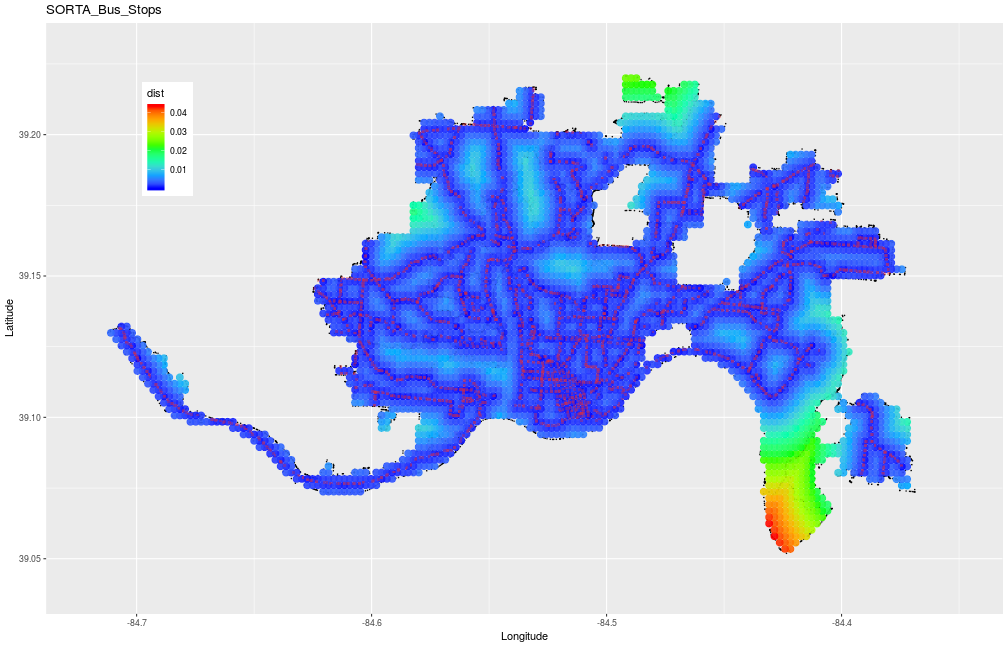
\includegraphics[height=3cm]{busStopDistance} \\
    \small A & \small B \
  \end{tabular}
\end{center}


\end{document}